\documentclass[12pt]{article}

\usepackage{listings}
\usepackage{amsmath}
\usepackage[top=5em, bottom=5em, left=5em, right=5em]{geometry}
\usepackage{tikz}
\usetikzlibrary{positioning}
\usetikzlibrary{shapes.geometric}

\setlength\parindent{0em}
\setlength\parskip{1em}

\title {Assignment 2}

\author {Hendrik Werner s4549775}

\begin{document}
\maketitle

This was done in collaboration with Constantin Blach (s4329872).

\section{} %1
Here is an implementation of a Queue using two stacks to store its elements written in Groovy:

\lstinputlisting{code/TwoStackQueue.groovy}

It can be used like this:

\begin{lstlisting}
def range = 1..10
TwoStackQueue<Integer> q = new TwoStackQueue()
for (int i in range) {
    q.add i
}
for (int i in range) {
    println q.get()
}
\end{lstlisting}

\section{} %2
Here is an imlpementation of a Deque using an array to store its elements written in Groovy:

\lstinputlisting{code/ArrayDeque.groovy}

Here is a usage example:

\begin{lstlisting}
def deque = new ArrayDeque<Integer>(2)
deque.addEnd(3)
deque.addStart(5)
println deque.removeStart()
println deque.removeEnd()
\end{lstlisting}

\section{} %3
Here is an implementation of a singly linked, circular list in written in Groovy:

\lstinputlisting{code/SinglyLinkedCircularList.groovy}

You could implement a method to delete the next element in $O(1)$. You could also implement a method to look at the next element in $O(1)$ to be able to use the $deleteNext$ method in a useful way.

\section{} %4
\section{} %5
A direct access table is a table of the same size as the key range. Its size does not change but it instead contains a field for every possible key. This makes insert, delete, get, search, etc. $O(1)$ operations.

When we want to find the maximum element we need to iterate over all entries and compare them to each other. The naive approach would take $O(m)$ time in the worst case (the maximum element is in the last field) where $m$ is the size of the table.

We could improve this by storing a list of used keys and only comparing the elements at those indexes to each other. This would bring the time complexity down to $O(k)$ where $k$ is the number of entries.

Given here is a description of the naive approach:

\begin{enumerate}
	\item Create a variable $max$ and set it to the fist element.
	\item Create a variable $next$
	\item \label{itm:loop} Check if there is a next element. If so, set $next$ to it. If not, return $max$.
	\item If $next > max$ then $max = next$.
	\item Go to step \ref{itm:loop}.
\end{enumerate}

\section{} %6
$h(k) = k \mod 7$

$h(12) = 5,$ $h(44) = 2,$ $h(13) = 6,$ $h(88) = 4$\\
$h(23) = 2,$ $h(94) = 3,$ $h(11) = 4,$ $h(39) = 4$\\
$h(20) = 6,$ $h(16) = 2,$ $h(5) = 5$

The slots are empty initally:
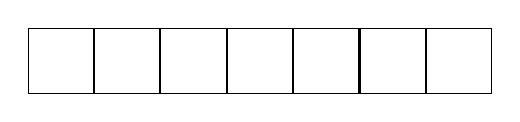
\begin{tikzpicture}[entry/.style={regular polygon, regular polygon sides=4, draw, text width=1em}]
	\node [entry] (a0_0) {};
	\node [entry, right=0em of a0_0] (a1_0) {};
	\node [entry, right=0em of a1_0] (a2_0) {};
	\node [entry, right=0em of a2_0] (a3_0) {};
	\node [entry, right=0em of a3_0] (a4_0) {};
	\node [entry, right=0em of a4_0] (a5_0) {};
	\node [entry, right=0em of a5_0] (a6_0) {};
\end{tikzpicture}

When we add an element to the table we store it at the index of its hash value. Example: $h(12) = 5$ so we store $12$ at index 5:

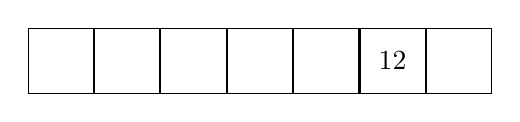
\begin{tikzpicture}[entry/.style={regular polygon, regular polygon sides=4, draw, text width=1em}]
	\node [entry] (a0_0) {};
	\node [entry, right=0em of a0_0] (a1_0) {};
	\node [entry, right=0em of a1_0] (a2_0) {};
	\node [entry, right=0em of a2_0] (a3_0) {};
	\node [entry, right=0em of a3_0] (a4_0) {};
	\node [entry, right=0em of a4_0] (a5_0) {12};
	\node [entry, right=0em of a5_0] (a6_0) {};
\end{tikzpicture}

When there are already elements stored at index 5 we need to resolve this collision. Here we use chaining as a resolution strategy. This means that when storing $5$ whose hash value is $h(5) = 5$ we will store it in a list node and point the last list node at index $5$ ($12$ in this case) to it:

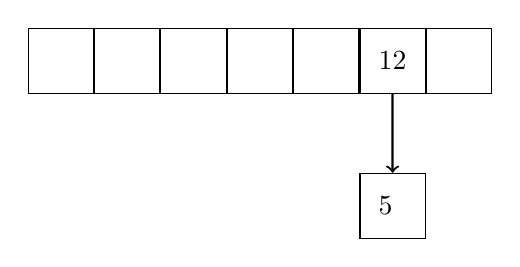
\begin{tikzpicture}[entry/.style={regular polygon, regular polygon sides=4, draw, text width=1em}]
	\node [entry] (a0_0) {};
	\node [entry, right=0em of a0_0] (a1_0) {};
	\node [entry, right=0em of a1_0] (a2_0) {};
	\node [entry, right=0em of a2_0] (a3_0) {};
	\node [entry, right=0em of a3_0] (a4_0) {};
	\node [entry, right=0em of a4_0] (a5_0) {12};
	\node [entry, right=0em of a5_0] (a6_0) {};

	\node [entry, below=of a5_0] (a5_1) {5};

	\draw[->, thick] (a5_0) -- (a5_1);
\end{tikzpicture}

After adding all the values the hash table looke like this:

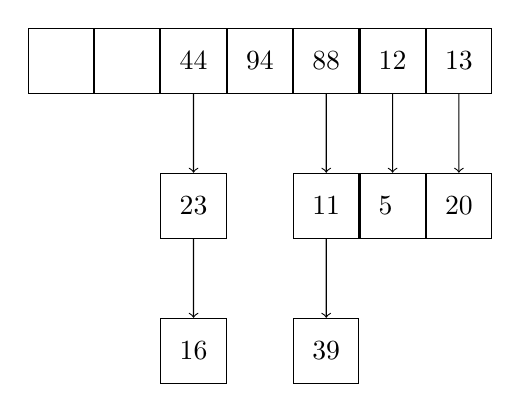
\begin{tikzpicture}[entry/.style={regular polygon, regular polygon sides=4, draw, text width=1em}]
	\node [entry] (a0_0) {};
	\node [entry, right=0em of a0_0] (a1_0) {};
	\node [entry, right=0em of a1_0] (a2_0) {44};
	\node [entry, right=0em of a2_0] (a3_0) {94};
	\node [entry, right=0em of a3_0] (a4_0) {88};
	\node [entry, right=0em of a4_0] (a5_0) {12};
	\node [entry, right=0em of a5_0] (a6_0) {13};

	\node [entry, below=of a2_0] (a2_1) {23};
	\draw[->] (a2_0) -- (a2_1);
	\node [entry, below=of a2_1] (a2_2) {16};
	\draw[->] (a2_1) -- (a2_2);
	\node [entry, below=of a4_0] (a4_1) {11};
	\draw[->] (a4_0) -- (a4_1);
	\node [entry, below=of a4_1] (a4_2) {39};
	\draw[->] (a4_1) -- (a4_2);
	\node [entry, below=of a5_0] (a5_1) {5};
	\draw[->] (a5_0) -- (a5_1);
	\node [entry, below=of a6_0] (a6_1) {20};
	\draw[->] (a6_0) -- (a6_1);
\end{tikzpicture}

\end{document}
